
% However, this does not guarantee the QoS of latency sensitive queries because of reasons such as resource interference and application scaling characteristics as discussed in Section \ref{sec:motivation}

Motivated by our five key observations for a robust GPU-aware orchestration layer, we built \textit{Knots} and integrate it with \textit{Kubernetes} enabling GPU-aware orchestration.

\subsection{Knots Design}
Recall that, in order to make an effective scheduling decision at the cluster-level for a heterogeneous cluster with GPUs, \textit{Kubernetes} needs to know the real-time utilization of the accelerator devices to schedule to a node that would guarantee the end-to-end container performance. To ensure this, we design \textit{Knots} to collect and log the real-time GPU utilization metrics through pyNVML~\cite{pynvml}, which is a Python-based API library that exposes utilization metrics to the node-level aggregator. As shown in Figure~\ref{fig:kubeknots}, we log the following five GPU metrics in real-time: (i) streaming multiprocessor (SM) utilization, (ii) memory utilization, (iii) power consumption, (iv)transfer bandwidth and, (v) receive bandwidth . These metrics are pushed to a node-level Influx-DB (IDB) \cite{InfluxDB} time-series database. \textit{Knots} in the head node can query the GPU nodes for utilization data via the utilization aggregator which is further explained in detail in Section \ref{sec:scheme}. The frequency at which the \textit{Knots} queries the IDB, determines the prediction accuracy and the quality of scheduling. When the pod is scheduled to the respective node, it pulls the docker image of the pod from a centralized docker image hub. From section~\ref{sec:TF-mem-sec}, we infer that memory utilization is a crucial metric, which \textit{Knots} leverages for container resizing and capacity provisioning. However, the other metrics like SM Utilization and I/O bandwidth are also used by the schedulers built leveraging \textit{Knots} discussed in further sections. 

\subsection{Representative GPU workload}
We next describe a representative workload that we use to capture the GPU context correctly. Since accelerators like GPUs in production datacenters are relatively recent, we wanted to faithfully capture the dynamics of applications that would be representative of a production datacenter load. As discussed in Section \ref{sec:motivation}, we choose eight scientific applications from the Rodinia benchmark suite~\cite{che2009rodinia} to represent the datacenter batch jobs. For user-facing services, we used a mix of DNN-based inference queries from Djinn and Tonic workload suite~\cite{hauswald2015djinn} (refer Table~\ref{tbl:appmix} \footnote{The abbreviations for application names can be found in \cite{hauswald2015djinn}}). 

We did initial performance characterization experiments to determine the performance demands to come up with three different bins based on load and covariance as shown in the Table~\ref{tbl:appmix}. As observed earlier from Figure \ref{fig:rodinia-peaks}, a batch application can subscribe to highly correlatable GPU resources such as SM, memory, and bandwidth. (e.g., at time quantum 450, all the three resources are highly utilized which is classified as HIGH load). We repeatedly schedule the same set of workloads within a bin and start logging the performance metrics once a steady state is achieved.  We co-locate both the batch and production jobs on ten nodes which have an Nvidia P100 GPU. These GPUs are attached to their respective CPU hosts, and the queries are scheduled from a head node (configuration details in Table~\ref{tbl:hw-config}).

\begin{figure}
  \centering
  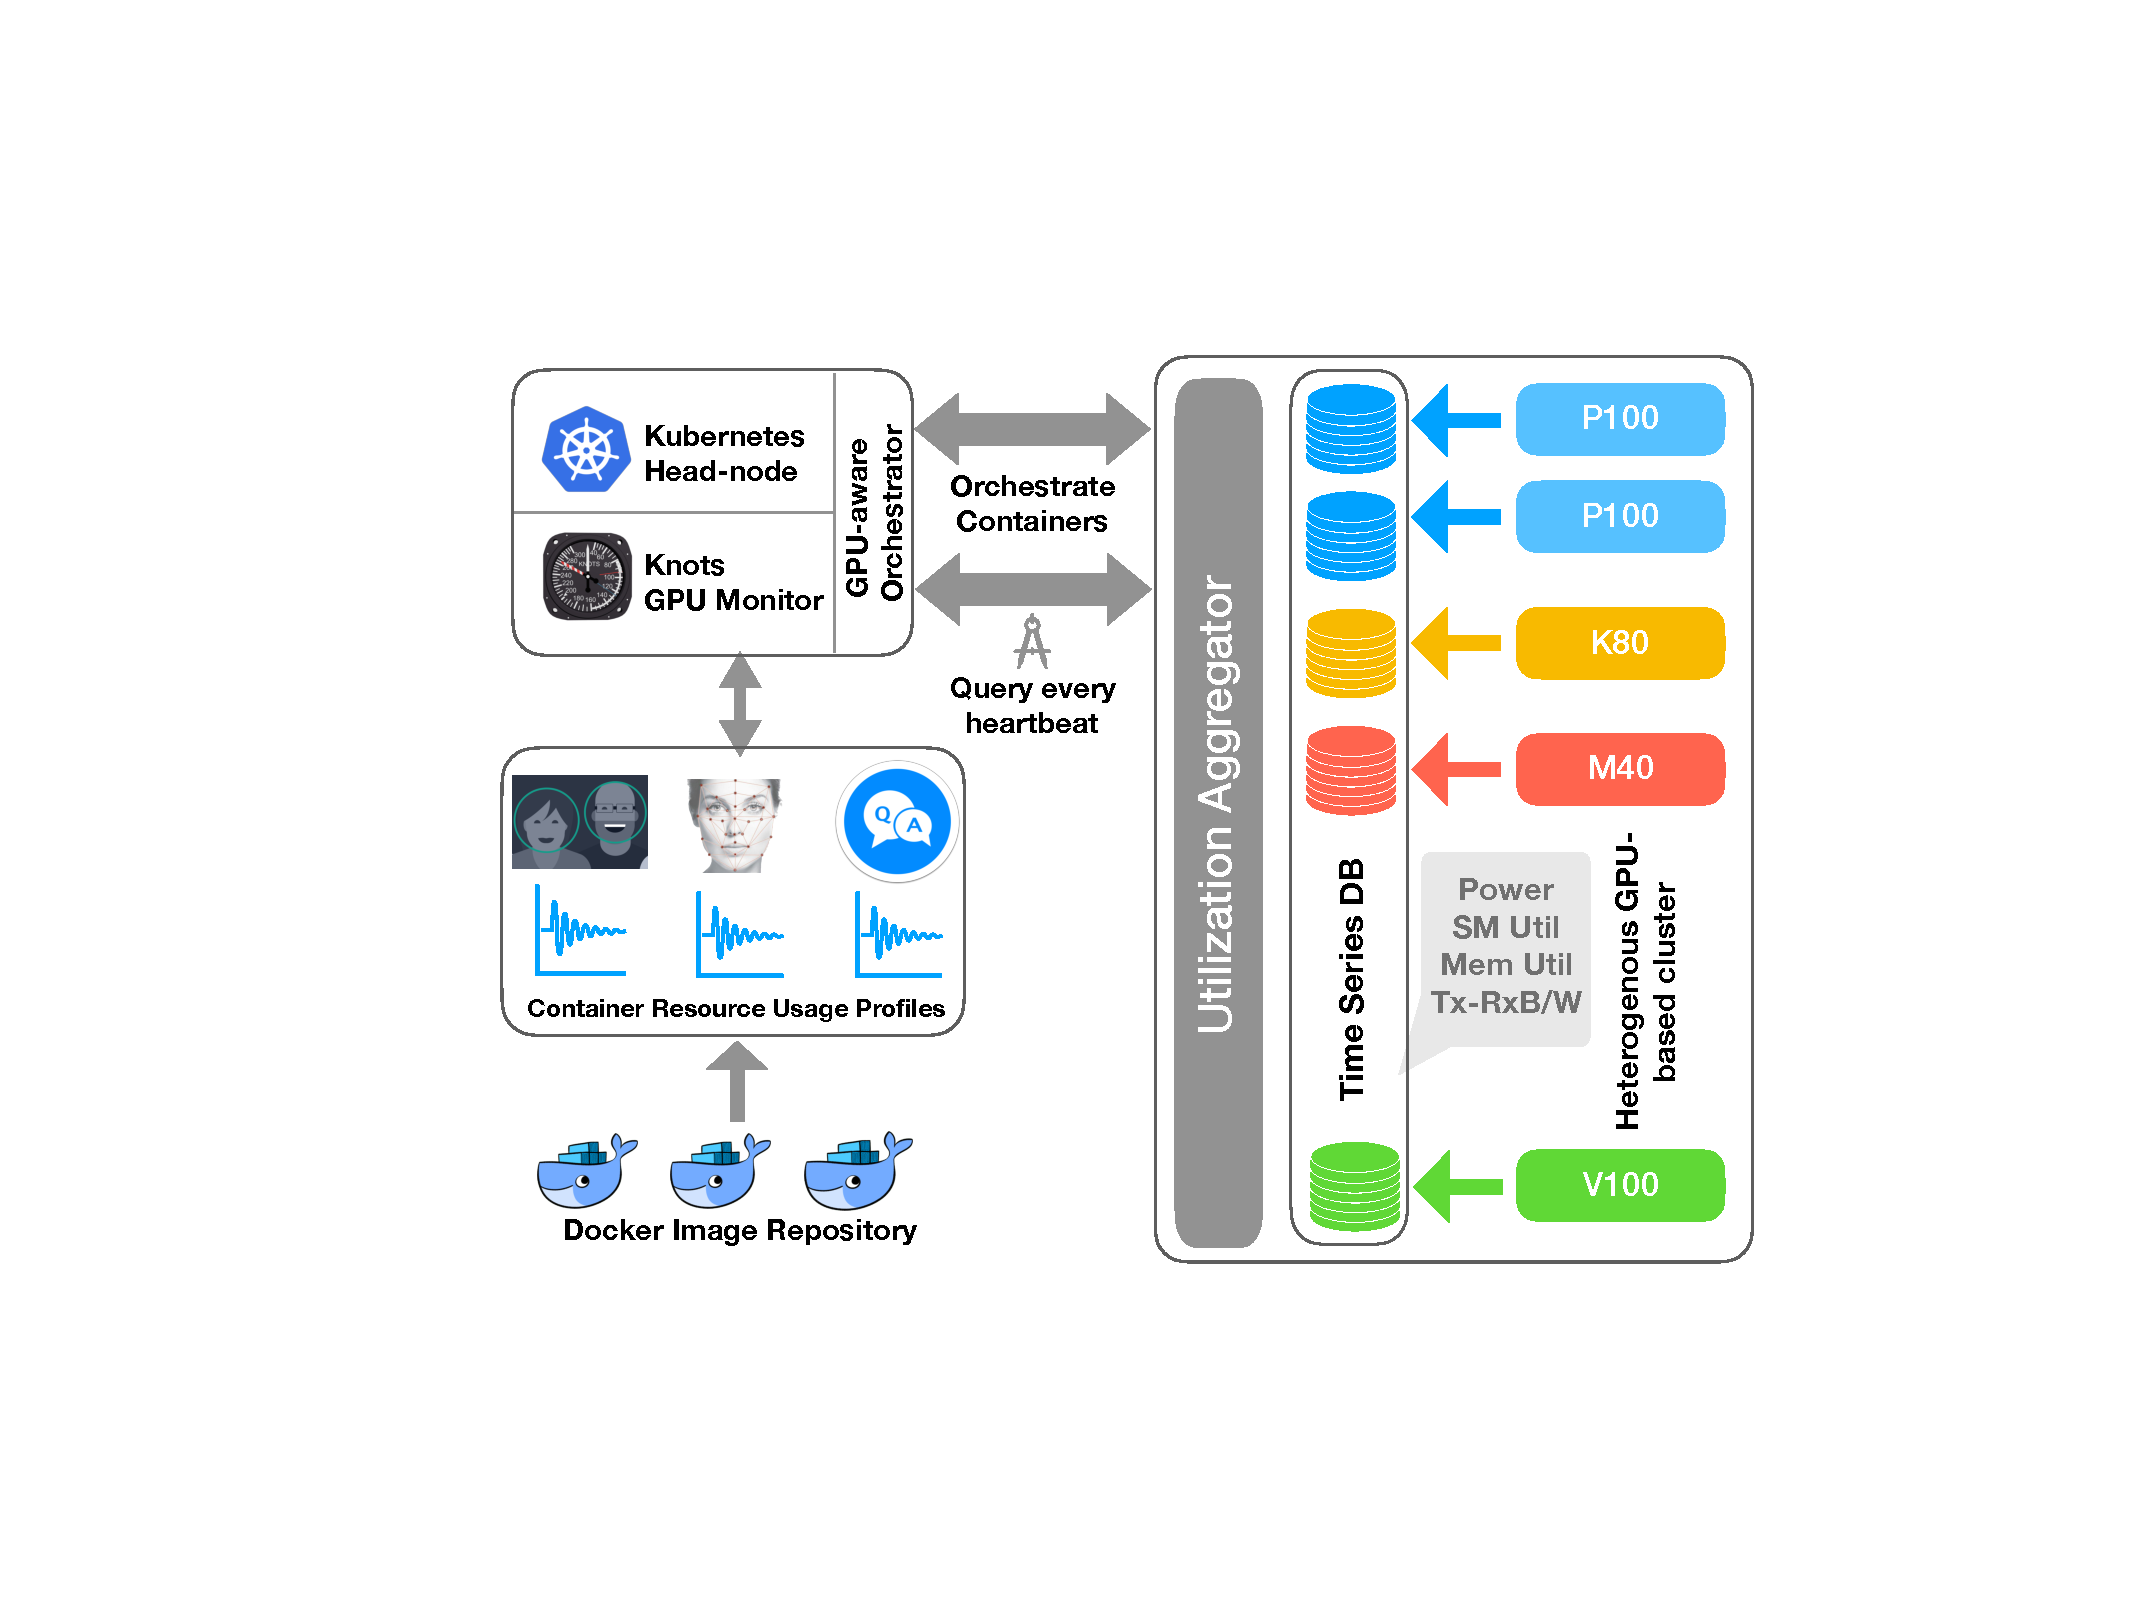
\includegraphics[width=.99\linewidth]{results/kube-knots.pdf}
  \caption{\textit{Kube-Knots} GPU orchestrator design.}
  \label{fig:kubeknots}
\end{figure}

% \vspace{-0.1in}
% \begin{center}
% \textit{The more you know about the past, the better prepared you are for the future - T. Roosevelt}
% \end{center}

\begin{table}[t]
%\setlength\extrarowheight{5pt}
% \begin{center}
\begin{minipage}{.99\linewidth}
\setlength\tabcolsep{1.1pt}
\resizebox{\textwidth}{!}{%
\renewcommand{\arraystretch}{1.2}
 \begin{tabular}{||c | c | c | c |c | c | c | c |c||} 
 \hline
 %\multicolumn{8}{|c|}{GPU Cluster Workload Mix} \\
 %\hline\hline
 \multicolumn{5}{|c|}{Batch workloads from Rodinia suite}&{Latency critical}&{Load}&{COV}\\
  \hline
  App-Mix-1 & leukocyte & heartwall & particlefilter & mummergpu & face,key & HIGH & LOW\\
 \hline
 App-Mix-2 & pathfinder & lud & kmeans & streamcluster & chl,ner,pos & MED & MED\\ 
 \hline
 App-Mix-3 & particlefilter & streamcluster & lud & myocyte & imc,face  & LOW & HIGH\\  
  \hline
\end{tabular}}
% \end{center}

\caption{GPU load and covariance for cluster workload suite mixed with batch jobs and latency critical ML inference queries.}
\vspace{-5mm}
\label{tbl:appmix}
\end{minipage}
\end{table}


\begin{figure*}[!tbp]
\begin{subfigure}[b]{0.33\textwidth}
  \centering
  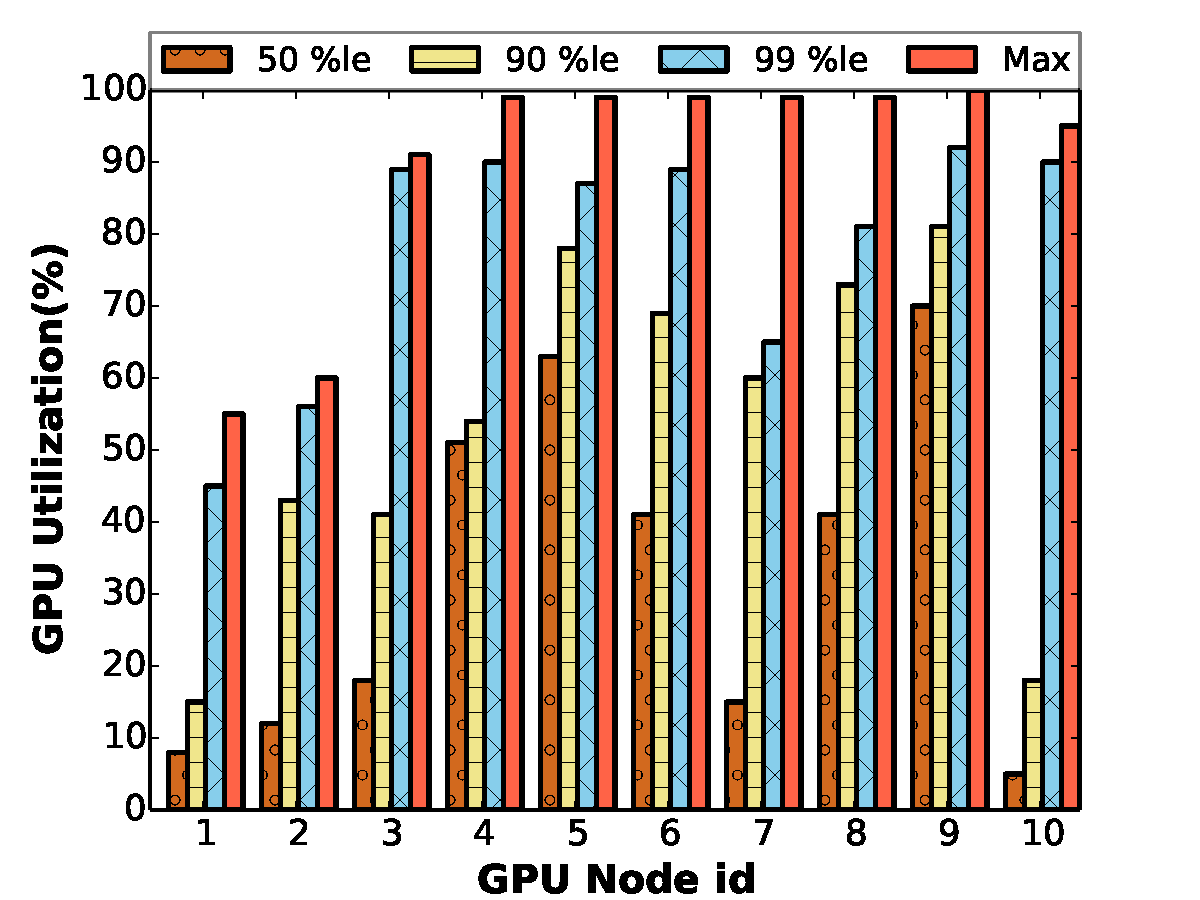
\includegraphics[width=1.1\linewidth]{results/app1-high.pdf}
  \caption{Application-Mix-1}
  \label{fig:app1}
\end{subfigure}
\begin{subfigure}[b]{.33\textwidth}
  \centering
  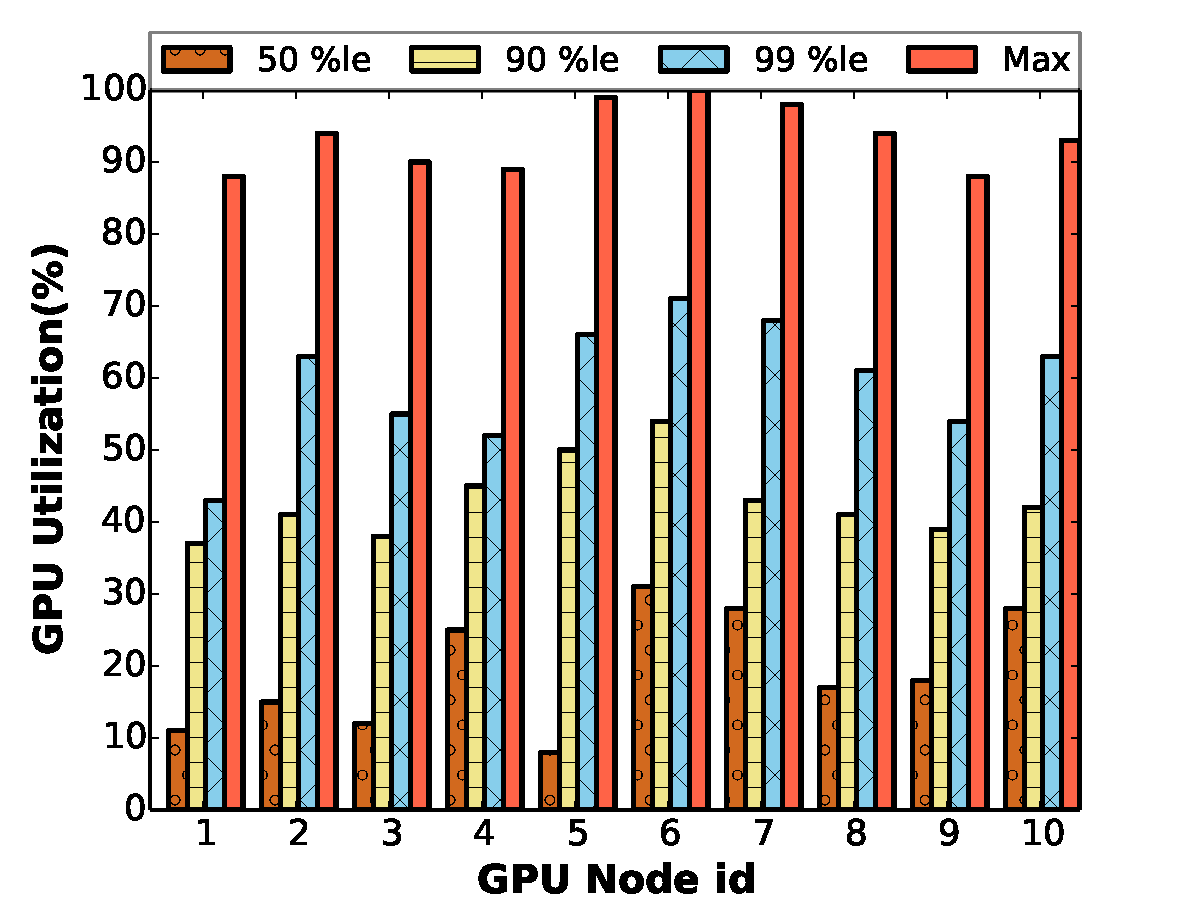
\includegraphics[width=1.1\linewidth]{results/app2-med.pdf}
  \caption{Application-Mix-2}
  \label{fig:app2}
\end{subfigure}
\begin{subfigure}[b]{.33\textwidth}
  \centering
  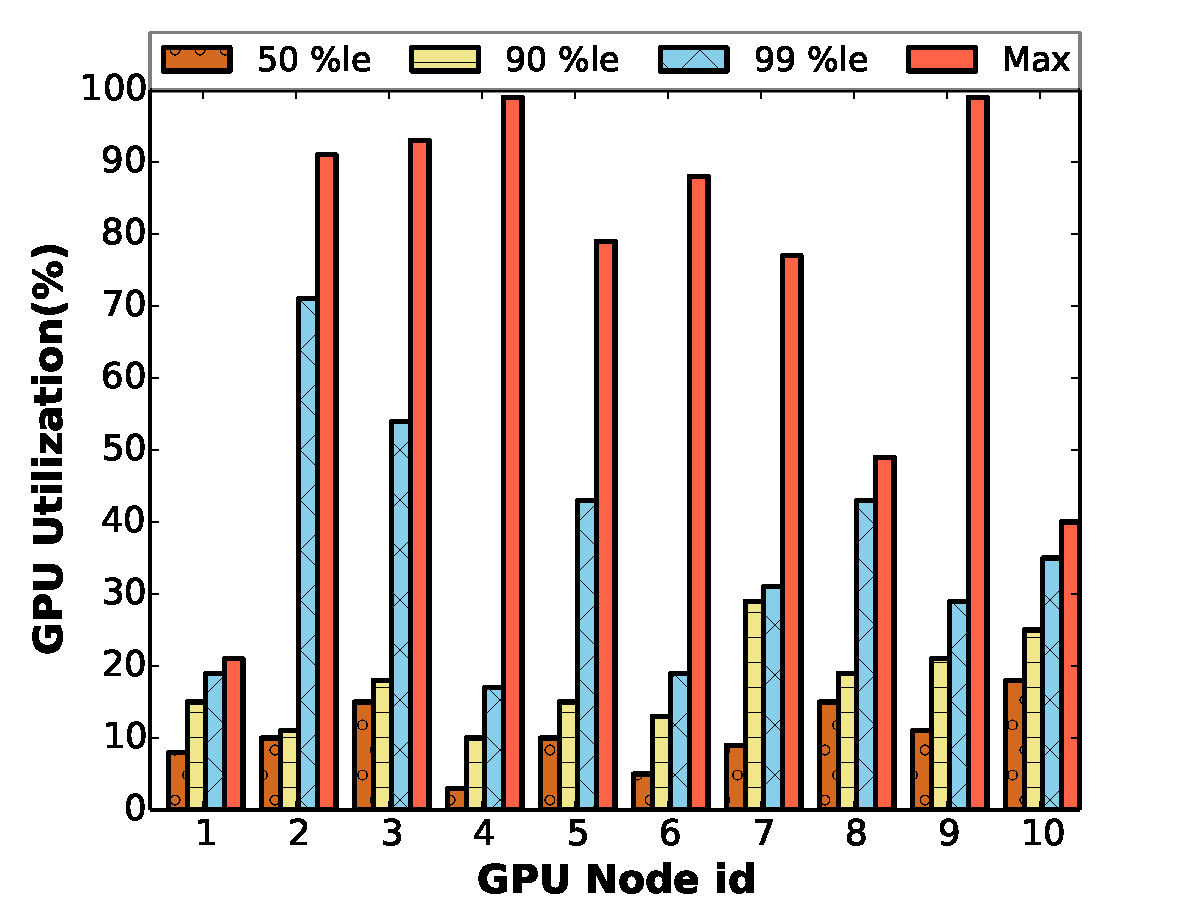
\includegraphics[width=1.1\linewidth]{results/app3-low.pdf}
  \caption{Application-Mix-3}
  \label{fig:app3}
\end{subfigure}
\vspace{-7mm}
\caption{50/90/99$^{th}$ percentile \& maximum GPU utilization for different application mixes scheduled using uniform scheduler.}
\label{fig:uniform}
\end{figure*}

\begin{figure}[tbp!]
\begin{subfigure}[b]{0.15\textwidth}
  \centering
  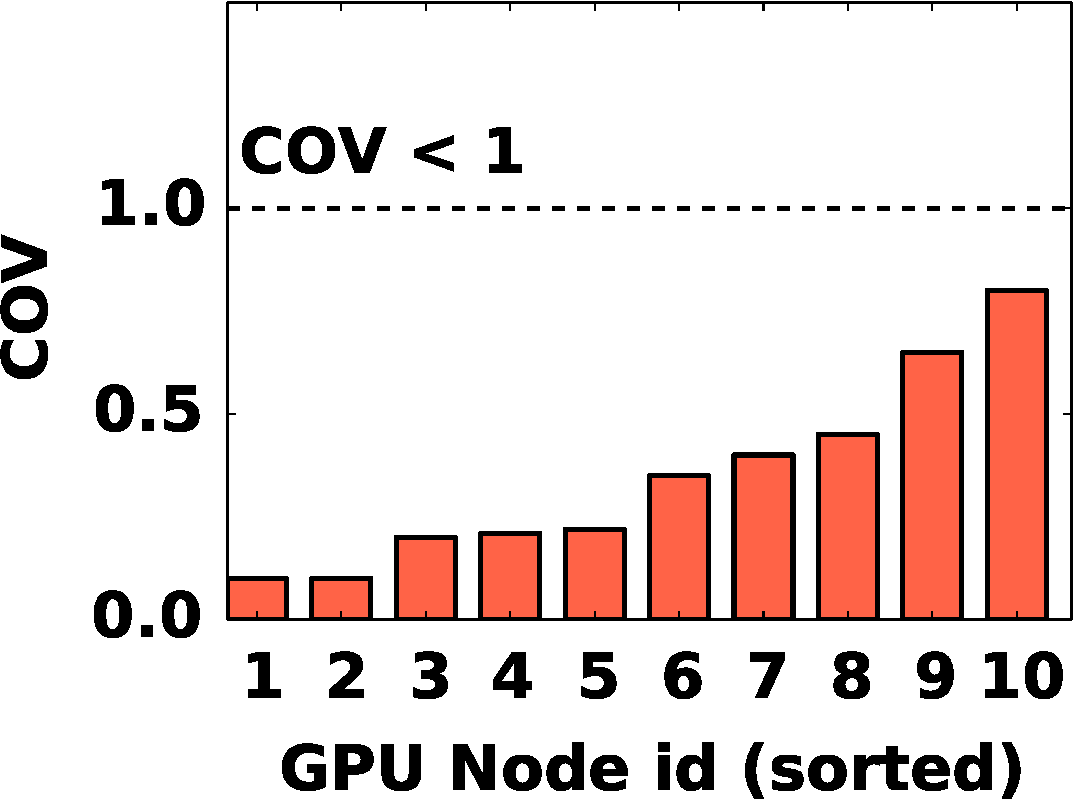
\includegraphics[width=.99\linewidth]{figs/app1-cov.pdf}
  \caption{App-Mix-1}
  \label{fig:app1-cov}
\end{subfigure}
\begin{subfigure}[b]{.15\textwidth}
  \centering
  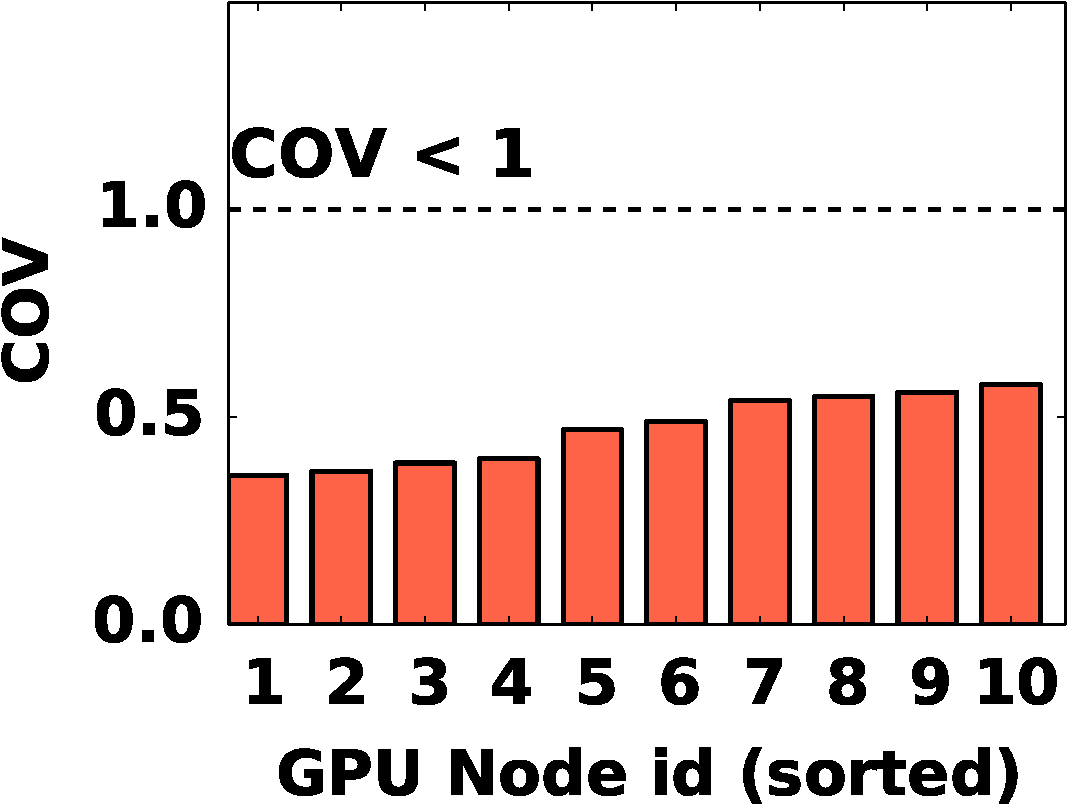
\includegraphics[width=.99\linewidth]{figs/app2-cov.pdf}
  \caption{App-Mix-2}
  \label{fig:app2-cov}
\end{subfigure}
\begin{subfigure}[b]{.15\textwidth}
  \centering
  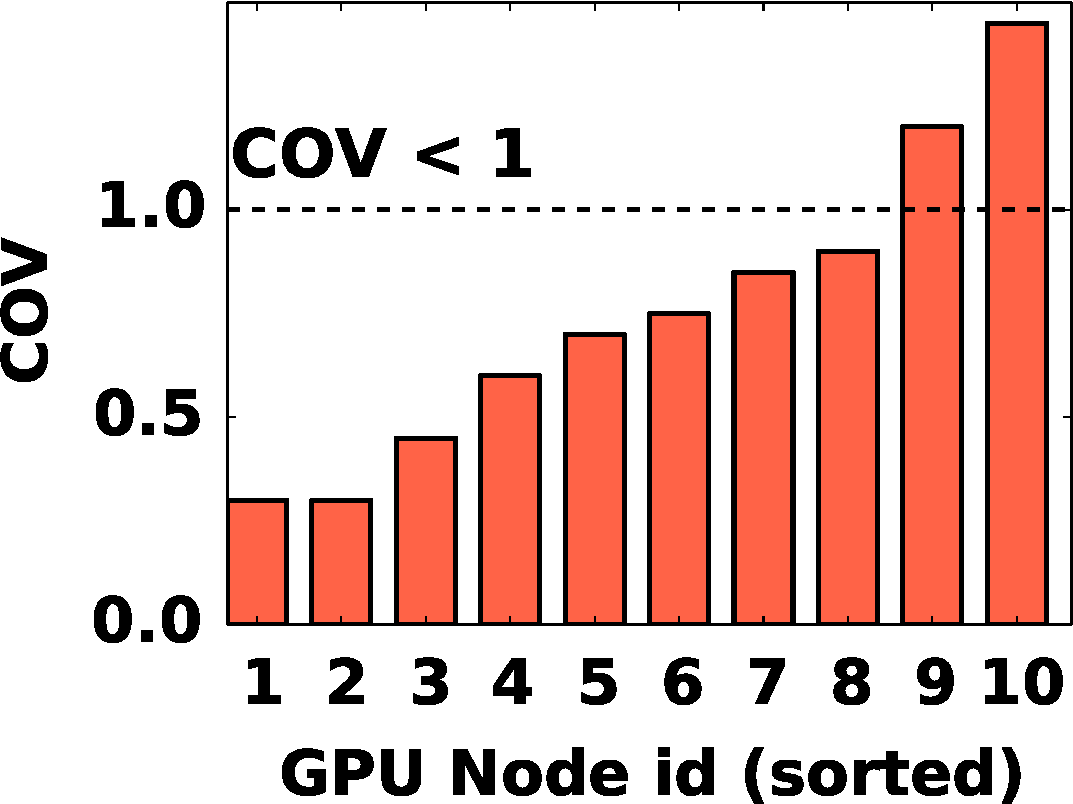
\includegraphics[width=.99\linewidth]{figs/app3-cov.pdf}
  \caption{App-Mix-3}
  \label{fig:app3-cov}
\end{subfigure}
\vspace{-2mm}
\caption{Coefficient of Variance across three Application-Mix.}
\label{fig:cov}
\end{figure}
\vspace{-2mm}


\subsection{Application-mix Analysis}
To schedule these workloads onto the GPU nodes, We use the \textit{Kubernetes} default scheduler, which uses the uniform scheduler to schedule containers and queries in FCFS basis. This scheduling policy is simple and scalable. It works well when the capacity of the resource is in abundance like CPUs. By default, GPU sharing is disabled as it complicates the scheduler-level performance/QoS guarantees and to ensure fairness across different co-scheduled applications. We schedule the app-mix through the uniform scheduler and plot the 50, 90, 99$^{th}$ percentile GPU utilization along with maximum utilization of individual GPUs as seen in Figure~\ref{fig:uniform}. For app-mix1 (in Figure \ref{fig:app1}) the 50$^{th}$ percentile utilization is much closer to 90$^{th}$/99$^{th}$ percentile utilization when compared to app-mix-3 (in Figure \ref{fig:app3}). This implies that the application load of app-mix-1 is \textit{higher} than app-mix-3, as we classified in Table \ref{tbl:appmix}. On the other hand, app-mix-2 in Figure \ref{fig:app2} has the 50\textsuperscript{th} to 99\textsuperscript{th} percentile evenly spaced. This also correlates to the classification we make for app-mix-2 in Table \ref{tbl:appmix} (indicates \textit{medium} load). %In these cases, both the 90,99$^{th}$\%le values are very close to the maximum GPU utilization. It also is critical to analyze the skew of the app-mix-3's utilization distribution in Fig~\ref{fig:app3}. It can be observed that the 50 and 90$^{th}$\%le GPU utilization is significantly less than 99$^{th}$\%le and the maximum utilization in most of the cases. This because the nature of the applications scheduled in this mix exhibit high variation in its resource demands though the aggregate utilization is low. This nature of the application also aligns with our observations made from Figure~\ref{fig:rodinia-peaks}. It is evident from these observations that the application usually overstates its resource requirements.

It is evident that, the applications have varying resource needs throughout their lifetime. Also, the applications always overstate their resource requirements by considering only for the peaks in the utilization  (also seen in Figure \ref{fig:rodinia-peaks}). This leads to under-utilization and queuing delays which directly results in poor energy efficiency and significant QoS violations, respectively. An efficient resource scheduler should leverage this dynamic workload behavior and incorporate policies that can guarantee the QoS while keeping the utilization high and improving energy efficiency. 

% If we could size an application based on 90-percentile CPU utilization instead of maximum CPU utilization, it could lead to significant savings. We also look at the other GPU utilization in Figure~\ref{fig:app2} and find that the observations to hold good even in case of average utilization.

\subsection{Utilization Variance Across GPU Nodes}
We also look into the variability in GPU utilization across the three different application mixes through the coefficient of variation(COV). COV is measured by the ratio of standard deviation $\sigma$ and mean $\mu$. This metric is a good indicator of the variations in the performance demands of the respective application mix. An application-mix with higher COV values are considered high in variance and harder to guarantee the performance when scheduled to the nodes. Consequently, those with COV$\leq$1 exhibit predictable workload consumption. It also makes it easier to guarantee the performance of an application to be scheduled to those nodes. Further, co-locating a heavy-tailed distribution (COV$\geq$1) to a positively correlated distribution with decaying tail (COV=1) would lead to application interference(noisy-neighbor) and severe capacity violations.
%\jash{relate noisy with spearman}

We sort the COV for all GPU nodes within an application mix and show it in Figure~\ref{fig:cov}. We observe that the COV is less than 1 for both app-mix-1 and app-mix-2. Therefore, it is easier to predict and guarantee while scheduling in those scenarios. In case of app-mix-3, the COV is greater than 1, and these applications have very low resource consumption. It is important for a GPU scheduler to take this into account while scheduling an application. If the scheduler is agnostic to the real-time utilization of the GPU, it will lead to co-location that results in heavy-tail distribution (e.g, time quantum 410-690 in Figure \ref{fig:rodinia-peaks}) resulting in pod failure. Hence it is important for a GPU orchestrator to provision for an application considering the real-time utilization metrics.
% hiding container launch latency while doing proactive admission control
% heterogeneous GPU allocation for bandwidth bound kernels to peak efficiency 
% inference workloads
% GPU performance prediction using ARIMA 
% Propose energy-aware scheduling schemes for tasks with energy constraints


% Node-level sharing related work comparison and problems
% Eg., non-preemptable accelerator issues demand smarter scheduling at first

% If shared what is the problem?
% Multi-container packing issues like memory crashing
% why? Underutilization of active memory across containers in GPU using 3 workloads
% Key factors: Memory,PCIe bandwidth,Queuing delay
% Predicting the container memory and saving container crashes

% Monitoring container usage on GPUs
% Proactive admission control and orchestration
% under-utilization, non pre-emptibility of GPUs, QoS guarentee, 
% Microservices and container framework

% Memory underutilization
% Energy
% exsiting TF library over commitment


%%%%%%%%%%%%%%%%
%\vspace{-0.15in}
